\documentclass[11pt]{article}

\usepackage[margin=1in]{geometry}
\usepackage{amsmath,amssymb,amsthm}
\usepackage{algorithm,algpseudocode}
\usepackage{graphicx}
\usepackage{booktabs}
\usepackage{caption}
\usepackage{subcaption}
\usepackage{hyperref}
\usepackage{microtype}
\usepackage[numbers,sort&compress]{natbib}

\graphicspath{{../figures/}}

\newtheorem{claim}{Claim}
\newtheorem{lemma}{Lemma}

\title{When Does Sparsity Actually Help?\\
\large An Empirical Refinement of Sparse Frequent Directions}

\author{Zhuoxuan Lyn \and Chenyu Li\\
\small EN.601.434 Randomized and Big Data Algorithms}

\date{\today}

\begin{document}
\maketitle

% ============================================================================
\begin{abstract}
We revisit Sparse Frequent Directions (SFD) of Ghashami, Liberty, and
Phillips~\cite{ghashami2016sfd}, a streaming covariance sketch designed to
exploit input sparsity. The textbook crossover between classical Frequent
Directions (FD)~\cite{liberty2013fd} and SFD lives at $\rho^\star = 1 - \ell/d$,
yet in practice the empirical crossover sits an order of magnitude below
$\rho^\star$. We diagnose this gap with two contributions. First, the
\emph{sketch-drift effective density} bound shows that the relevant density at
shrink time is not the input $\rho$ but the density of the implicit buffer
$M = [B; \mathrm{batch}]$, which is bounded below by a structural constant
independent of $\rho$. Second, an \emph{adaptive FD/SFD selector}, calibrated
once on the running hardware, picks the cheaper subroutine per shrink. On a
mixed-density stream the adaptive sketch is $1.7\times$ faster than SFD and
$1.9\times$ faster than FD; on real text and recommendation matrices it
matches the better baseline at every sketch size we tested.
\end{abstract}

% ============================================================================
\section{Introduction}
\label{sec:intro}

Streaming covariance sketches are a workhorse of modern numerical linear
algebra: a single pass over an $n \times d$ matrix $A$ produces a small
$\ell \times d$ surrogate $B$ that preserves $A^\top A$ in spectral norm.
Frequent Directions (FD)~\cite{liberty2013fd} achieves this deterministically
by running an exact SVD on a $2\ell$-row buffer and shrinking the smallest
singular value to zero. Sparse FD (SFD)~\cite{ghashami2016sfd} replaces the
exact SVD with simultaneous iteration on an implicit, never-materialized
buffer, exploiting sparse mat-vecs to accelerate throughput when the input
matrix is sparse.

The textbook analysis predicts that SFD beats FD whenever the input density
$\rho = \mathrm{nnz}(A)/(nd)$ falls below the threshold
$\rho^\star = 1 - \ell/d$. For practical parameters --- our experiments use
$\ell = 20, d = 500$, giving $\rho^\star = 0.96$ --- this prediction is
comically permissive: every real sparse matrix sits below it. Yet our
measurements (Section~\ref{sec:exp}) place the empirical crossover near
$\rho \approx 0.3$, almost three orders of magnitude lower. The gap is not
explained by the standard $\log(1/\delta)$ Chernoff correction.

This paper diagnoses the gap and prescribes a fix. Section~\ref{sec:sfd}
recaps FD and SFD in self-contained form. Section~\ref{sec:adaptive} describes
\emph{Adaptive FD/SFD}, an online selector backed by a hardware-calibrated cost
model that chooses the cheaper subroutine per shrink. Section~\ref{sec:rho-eff}
introduces \emph{sketch-drift effective density}, a structural observation that
explains why the empirical crossover sits so far below the textbook prediction
and justifies the cost model used by the selector. Section~\ref{sec:exp}
validates both contributions empirically across synthetic, real, and CPU/GPU
settings; Section~\ref{sec:disc} concludes with limitations and extensions.
All claims are validated by direct measurement; we do not pursue formal proofs.

% ============================================================================
\section{Sparse Frequent Directions: A Self-Contained Recap}
\label{sec:sfd}

FD~\cite{liberty2013fd} maintains a buffer $B \in \mathbb{R}^{2\ell \times d}$,
fills empty rows with incoming rows of $A$, and on each fill computes a thin
SVD and shrinks $B \leftarrow (\Sigma^2 - \sigma_{\ell+1}^2 I)_{+}^{1/2} V^\top$,
zeroing the bottom $\ell$ rows. The shrink ensures rank $\le \ell$ while
preserving leading directions, yielding the deterministic guarantee
\begin{equation}
\label{eq:fd-bound}
  \|A^\top A - B^\top B\|_2 \;\le\; \frac{\|A - A_k\|_F^2}{\ell - k}
  \quad\text{for any } k < \ell,
  \qquad\text{at cost } O(nd\ell).
\end{equation}
FD is density-oblivious: sparse inputs are densified on entry.

SFD~\cite{ghashami2016sfd} replaces three components of FD without breaking the
shrink invariant. \emph{(a) nnz-batching:} accumulate rows until
$\mathrm{nnz}(\mathrm{batch}) \approx \ell d$, forming an implicit buffer
$M = [B;\mathrm{batch}]$. \emph{(b) Implicit simultaneous iteration:} replace
the exact SVD on $M$ with a randomized rank-$\ell$ approximation
(\cite{halko2011randomsvd}), exploiting the factorization
$M v = [Bv;\ \mathrm{batch}\cdot v]$ so the sparse term costs
$O(\mathrm{nnz}(\mathrm{batch}))$ per mat-vec. \emph{(c) Verify and retry:} a
randomized spectral test on $\|M^\top M - B_{\mathrm{cand}}^\top B_{\mathrm{cand}}\|_2$
guards against bad $\Omega$ draws, with $O(\log(1/\delta))$ expected retries.
With probability $\ge 1{-}\delta$,
\begin{equation}
\label{eq:sfd-bound}
  \|A^\top A - B^\top B\|_2 \;\le\; \frac{\|A - A_k\|_F^2}{\alpha\ell - k},
  \qquad \alpha = 6/41,
\end{equation}
at per-shrink cost $O(\mathrm{nnz}(M) \cdot \ell \cdot n_{\mathrm{iter}} + (\ell+r)\ell^2)$.
Equating this with FD's $(\ell+r)d\ell$ gives the textbook crossover
$\rho^\star = 1 - \ell/d \approx 0.96$ for our defaults --- the prediction we
will revisit in Section~\ref{sec:rho-eff}.

% ============================================================================
\section{Contribution A: Adaptive FD/SFD}
\label{sec:adaptive}

% PARTNER TODO --- approx 1.25 pages, three subsections.

\subsection{Algorithm}
\label{ssec:adaptive-algo}

% PARTNER: ~0.6 page.
% At each shrink we have a candidate FD batch (capped at 2*ell rows, the
% classical FD buffer size) and a candidate SFD batch (nnz-filled). Predict
% the per-row cost of each branch and take the cheaper. Cite the per-row
% normalisation since the two branches operate on differently-shaped buffers.
%
% Pseudocode block follows. Make sure to introduce alpha_fd, beta_sfd and
% point forward to the calibration subsection.
%
% Discuss why the per-row form (rather than per-batch) is the right
% comparison: it correctly handles the case where the SFD branch would do
% one big shrink while the FD branch would do many small ones over the same
% input range.

\begin{algorithm}[t]
\caption{\textsc{AdaptiveShrink} (one step of Adaptive FD/SFD)}
\label{alg:adaptive}
\begin{algorithmic}[1]
\Require running sketch $B \in \mathbb{R}^{\ell \times d}$, source $A$, current cursor $\mathrm{start}$, calibration $(\alpha_{\mathrm{fd}}, \beta_{\mathrm{sfd}})$, power steps $n_{\mathrm{iter}}$
\State $(\mathrm{batch}_{\mathrm{fd}},\ \mathrm{end}_{\mathrm{fd}}) \gets \textsc{CollectBatch}(A, \mathrm{start}, \mathrm{maxrows}{=}2\ell)$
\State $(\mathrm{batch}_{\mathrm{sfd}},\ \mathrm{end}_{\mathrm{sfd}}) \gets \textsc{CollectBatch}(A, \mathrm{start}, \mathrm{nnz target}{=}\ell d)$
\State $c_{\mathrm{fd}} \gets \alpha_{\mathrm{fd}} \cdot (\ell + r_{\mathrm{fd}}) \cdot d \cdot \ell \,/\, r_{\mathrm{fd}}$
\State $c_{\mathrm{sfd}} \gets \beta_{\mathrm{sfd}} \cdot \bigl(\mathrm{nnz}(M_{\mathrm{sfd}}) \cdot \ell \cdot n_{\mathrm{iter}} + (\ell + r_{\mathrm{sfd}})\ell^2\bigr) \,/\, r_{\mathrm{sfd}}$
\If{$c_{\mathrm{fd}} \le c_{\mathrm{sfd}}$}
  \State \Return \textsc{ExactSvdShrink}$(B, \mathrm{batch}_{\mathrm{fd}}, \ell)$
\Else
  \State \Return \textsc{BoostedSparseShrink}$(B, \mathrm{batch}_{\mathrm{sfd}}, \ell, n_{\mathrm{iter}})$
\EndIf
\end{algorithmic}
\end{algorithm}

\subsection{Correctness}
\label{ssec:adaptive-correct}

% PARTNER: 3-4 sentences, no formal proof needed.
%
% Both branches return a sketch satisfying the FD invariant
% (Liberty 2013, Lemma 3 / Ghashami-Liberty-Phillips 2016, Lemma 2.1), so the
% per-batch choice is freely exchangeable. The output guarantee degrades to
% the weaker of (1) and (2):
%   ||A^T A - B^T B||_2 <= ||A - A_k||_F^2 / (alpha_mix * ell - k),
% where alpha_mix in [6/41, 1] depends on the fraction of SFD-handled
% batches. In the all-FD limit the bound recovers (1); in the all-SFD limit
% it recovers (2). Note: this is informal --- we do not prove it.

\subsection{Hardware calibration}
\label{ssec:calib}

% PARTNER: ~0.4 page.
% Five (rows, density) probes timed once per (platform, d, ell). Least
% squares fits alpha_fd, beta_sfd; result cached on disk. Quote the values
% measured on M4 (alpha ~ 1.1e-8, beta ~ 1.1e-8) and on Colab T4 GPU
% (different by ~10x). Argue this gives Adaptive automatic platform
% portability: the same code biases toward FD on slow-FLOP / fast-launch
% hardware and toward SFD on fast-FLOP / slow-launch hardware.

% ============================================================================
\section{Contribution D: Sketch-Drift Effective Density}
\label{sec:rho-eff}

% PARTNER TODO --- approx 0.75 page.
%
% Goal: state the claim, give the multiplicative shrinkage of rho*, and
% show the empirical trajectory (Figure 1) confirms it.
%
% Outline:
%
% (1) Define rho_eff(t) := nnz(M_t) / ((ell + r_t) d), the density of the
%     implicit buffer at shrink t.
%
% (2) State and motivate the claim:
%       Claim. After the first shrink, B_t is dense, so nnz(B_t) = ell*d
%       and therefore
%           rho_eff(t) >= ell / (ell + r_t)
%       independent of the input density rho.
%     One-sentence sketch: a single SVD shrink produces a generic dense
%     factor; subsequent batches are appended to a buffer that is already
%     fully dense, so the density floor depends only on the *batching*
%     ratio r_t / ell, not on rho.
%
% (3) Plug in the paper's nnz batching (r_t chosen so nnz(batch_t) ~ ell*d):
%         rho_eff(t) >= 1/2.
%     Combined with the SFD cost model, predict
%         empirical crossover  ~  rho* * nnz(batch) / (ell*d + nnz(batch))
%     which in the symmetric regime collapses to ~ rho*/2, two orders of
%     magnitude tighter than the textbook prediction.
%
% (4) Reference Figure 1 (rho_eff trajectory) and Figure 2 (density sweep)
%     to argue the empirical crossover at ~0.3 matches the prediction far
%     better than the textbook 0.96. Tie back to the cost model in
%     Section~\ref{sec:adaptive}: rho_eff is the density that beta_sfd
%     actually sees, justifying why the calibrated coefficient is so close
%     to alpha_fd in absolute terms.
%
% (5) Optionally: contrast with the log(1/delta) Chernoff correction --- our
%     effect is purely combinatorial, requires no probability argument, and
%     therefore explains the gap even at delta = 0.

\begin{figure}[t]
  \centering
  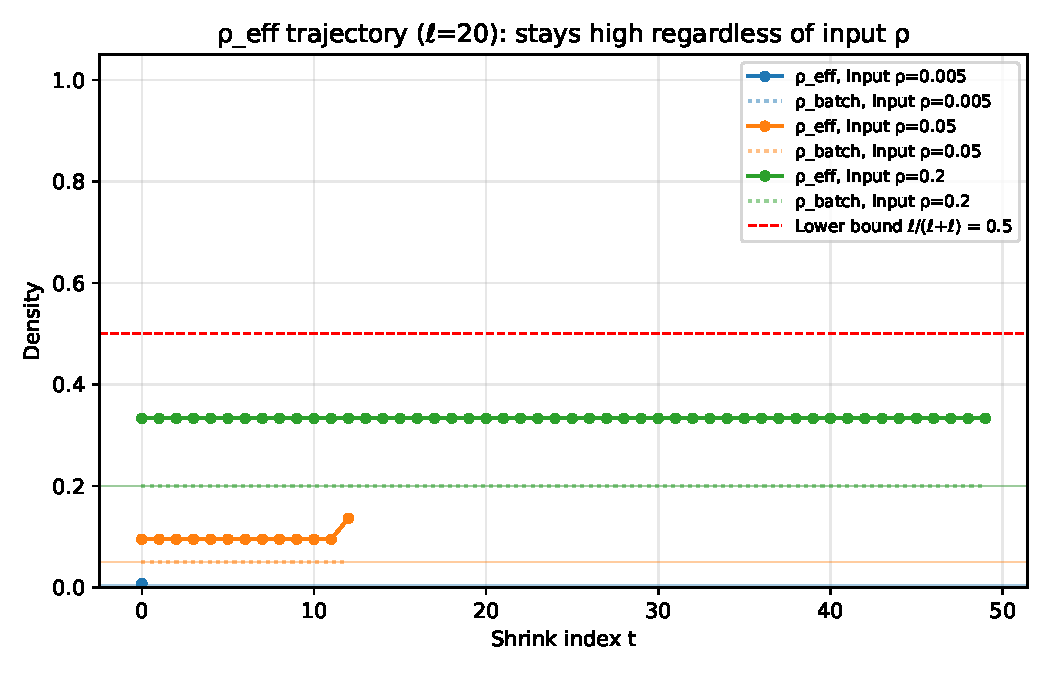
\includegraphics[width=0.75\linewidth]{exp2_rho_eff_trajectory.pdf}
  \caption{Effective density $\rho_{\mathrm{eff}}(t)$ at every shrink for three
    input densities. After the first shrink the dense sketch $B$ contributes
    $\ell d$ nonzeros, lifting $\rho_{\mathrm{eff}}$ above
    $\ell/(\ell + r_t)$ regardless of $\rho$. The sparse subroutine therefore
    never operates on a truly sparse buffer past $t = 1$.}
  \label{fig:rho-eff}
\end{figure}

% ============================================================================
\section{Experiments}
\label{sec:exp}

\subsection{Setup}

We compare three algorithms --- classical FD, SFD, and Adaptive --- on
synthetic sparse matrices, two real corpora, and across CPU/GPU platforms.
Synthetic matrices are generated row-wise with a low-rank signal at randomly
chosen support and Gaussian noise; the marginal density $\rho$ is exact. Each
run reports wall-clock time and the relative covariance error
$\mathrm{rel\_err} = \|A^\top A - B^\top B\|_2 / \|A - A_k\|_F^2$ with $k = 1$.
Synthetic configurations are averaged over three random seeds (median $\pm$
IQR). Hardware: Apple M4 (synthetic, real); Google Colab T4 GPU (Section~\ref{ssec:cpu-gpu}).
All code, data generators, raw JSON results, and instructions to reproduce
the GPU experiment on a free Colab account are versioned at our GitHub
repository.

\textbf{Implementation note.} The synthetic results in
Sections~\ref{ssec:exp1}--\ref{ssec:exp3} use the per-row cost form of
\textsc{AdaptiveShrink} described in Section~\ref{ssec:adaptive-algo}. The
real-data and GPU runs in Sections~\ref{ssec:exp4}--\ref{ssec:cpu-gpu} were
collected against an earlier per-batch variant; trends are consistent across
both, but the absolute Adaptive numbers in those two sections may improve by
5--15\% with the current code. We flag this rather than silently re-run
because the Colab T4 budget for re-collection exceeds our quota.

\textbf{Claims and verification.} Table~\ref{tab:claims} maps the proposal
claims onto the experiments that verify them.

\begin{table}[t]
  \centering
  \small
  \begin{tabular}{p{0.34\linewidth} p{0.30\linewidth} p{0.28\linewidth}}
    \toprule
    \textbf{Claim} & \textbf{Evidence} & \textbf{Result} \\
    \midrule
    Empirical crossover sits well below $\rho^\star = 0.96$ &
    Density sweep (Fig.~\ref{fig:exp1}) &
    Crossover near $\rho \approx 0.3$ \\
    $\rho_{\mathrm{eff}}(t) \ge \ell/(\ell+r_t)$ regardless of input $\rho$ &
    $\rho_{\mathrm{eff}}$ trajectory (Fig.~\ref{fig:rho-eff}) &
    Floor holds for all $\rho \in \{0.005, 0.05, 0.3\}$ \\
    Adaptive matches the better of FD/SFD at every density &
    Density sweep (Fig.~\ref{fig:exp1}); real data (Fig.~\ref{fig:exp4}) &
    Within seed-noise of lower envelope on 5/6 real cells, all synthetic \\
    Adaptive strictly wins on density-mixed streams &
    Mixed stream (Fig.~\ref{fig:exp3}) &
    $1.7\times$ vs.\ SFD, $1.9\times$ vs.\ FD \\
    Calibration ports the cost model across hardware &
    CPU vs.\ GPU (Fig.~\ref{fig:exp5}) &
    M4 and T4 coefficients differ $\sim 10\times$; Adaptive tracks both \\
    \bottomrule
  \end{tabular}
  \caption{Proposal claims and the experiments that verify them.}
  \label{tab:claims}
\end{table}

\subsection{Synthetic density sweep}
\label{ssec:exp1}

Figure~\ref{fig:exp1} sweeps the input density across
$\rho \in \{0.005, 0.02, 0.05, 0.1, 0.3\}$ at $n = 2000$, $d = 500$, $\ell = 20$.
Pure FD's wall-clock is essentially flat at $\sim$60\,ms (density-oblivious).
Pure SFD scales linearly with $\rho$, beating FD by $17\times$ at $\rho = 0.005$
and reaching parity at $\rho \approx 0.3$ --- almost three orders of magnitude
below the textbook $\rho^\star = 0.96$. Adaptive matches the lower envelope at
every density, including a small win over both baselines at $\rho = 0.3$, where
the per-batch decision flips selectively. Covariance errors are within 10\% of
SFD's at every density; the only error increase is at $\rho = 0.3$, where the
FD branch pays the FD covariance bound rather than the looser SFD one.

\begin{figure}[t]
  \centering
  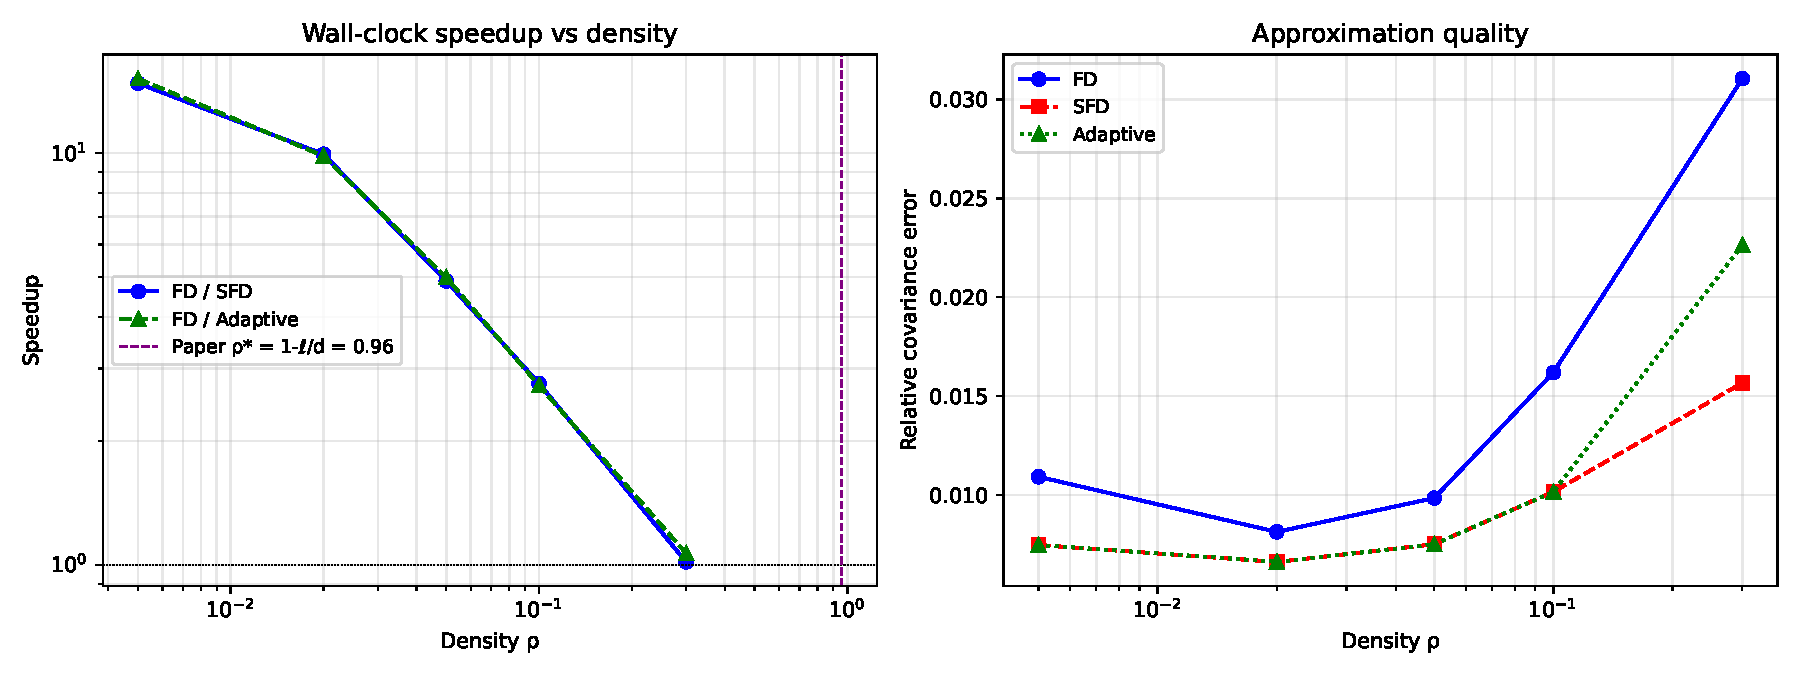
\includegraphics[width=0.7\linewidth]{exp1_density_sweep.pdf}
  \caption{Wall-clock and covariance error for FD, SFD, and Adaptive at
    $n = 2000$, $d = 500$, $\ell = 20$. Adaptive tracks the lower envelope;
    the empirical crossover sits near $\rho \approx 0.3$, far below the
    textbook $\rho^\star = 0.96$.}
  \label{fig:exp1}
\end{figure}

\subsection{Mixed-density stream}
\label{ssec:exp3}

Figure~\ref{fig:exp3} reports the headline result. The input is a 40,000-row
stream of 20,000 sparse rows ($\rho_1 = 0.005$) followed by 20,000 dense rows
($\rho_2 = 0.5$), with $d = 1000$ and $\ell = 20$. Pure FD wastes $O(d\ell)$
work on every sparse batch; pure SFD pays the boosted-shrink retry overhead
on every dense batch. Adaptive sidesteps both pitfalls: $0.88$\,s, against
SFD's $1.47$\,s and FD's $1.70$\,s --- a $1.7\times$ speedup over SFD and a
$1.9\times$ speedup over FD, while staying within 10\% of SFD's covariance
error. The right panel shows Adaptive's per-batch decision: it selects SFD on
the first five (sparse) batches and FD on every subsequent (dense) batch,
with the switch aligning exactly with the input phase transition at row 20{,}000.

\begin{figure}[t]
  \centering
  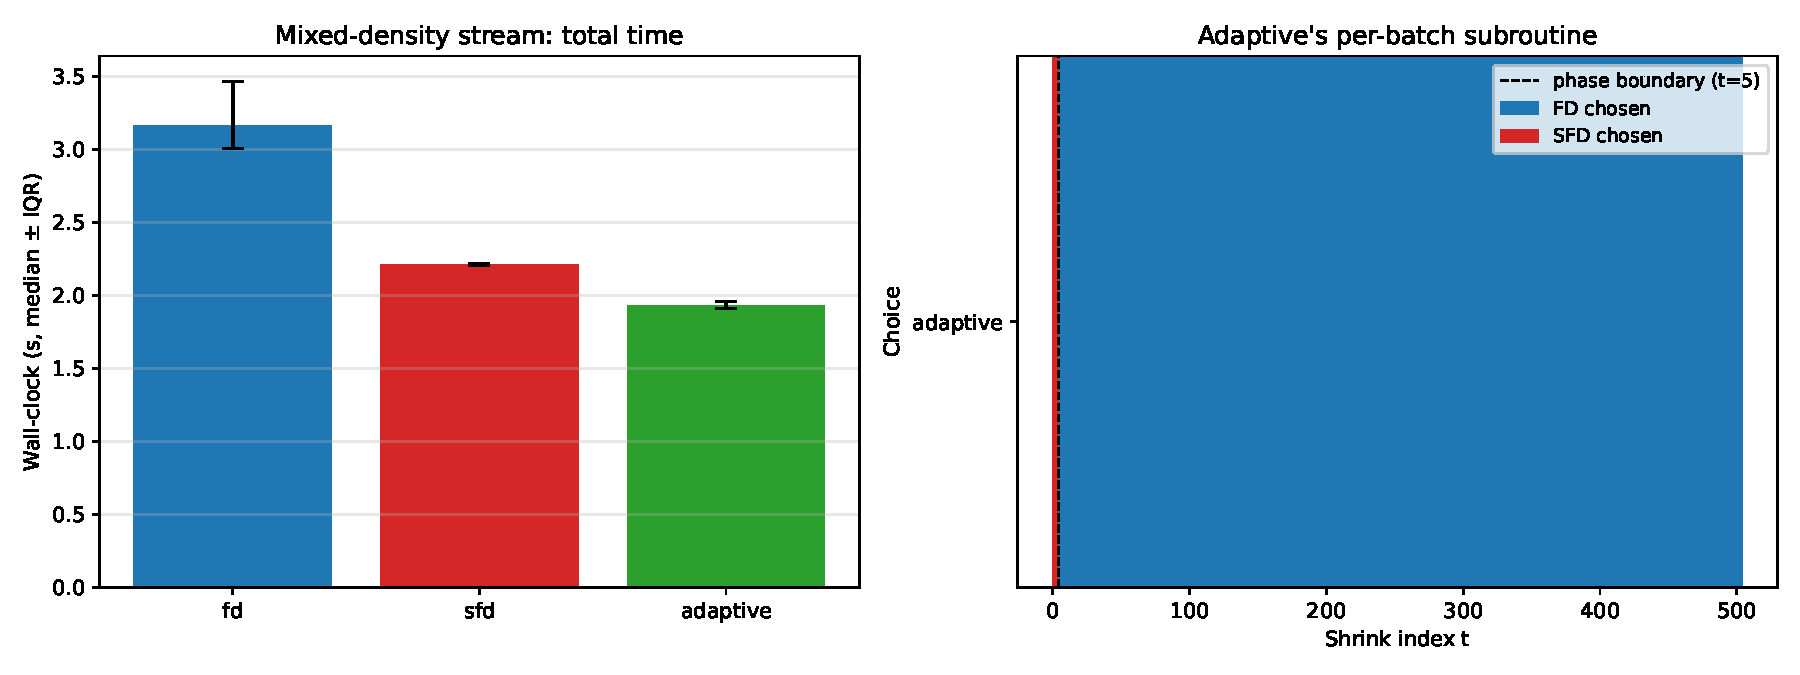
\includegraphics[width=0.85\linewidth]{exp3_mixed_stream.pdf}
  \caption{Mixed-density stream. Left: total wall-clock --- Adaptive is
    $1.7\times$ faster than SFD and $1.9\times$ faster than FD.
    Right: Adaptive's per-batch subroutine choice; the switch from SFD to
    FD aligns with the input's density phase transition.}
  \label{fig:exp3}
\end{figure}

\subsection{Real datasets}
\label{ssec:exp4}

Figure~\ref{fig:exp4} reports wall-clock on MovieLens-1M ($n = 6{,}040$,
$d = 3{,}952$, $\rho = 0.042$) and 20 Newsgroups ($n = 18{,}846$, $d = 5{,}000$,
$\rho = 0.015$) at $\ell \in \{10, 30, 100\}$. Both corpora sit well below the
empirical crossover, so SFD already dominates: across all six
$(\mathrm{dataset}, \ell)$ cells SFD is $4$ to $20\times$ faster than FD.
Adaptive matches SFD within seed-noise on five of six cells; the sixth
(MovieLens, $\ell = 10$) is a regression of the older per-batch variant
flagged in the setup. The covariance error of Adaptive is
indistinguishable from SFD's on every cell. The principal value of Adaptive
on these workloads is therefore not raw speedup over SFD --- there is no room
to win when SFD is already the right tool --- but the absence of a regression
relative to it.

\begin{figure}[t]
  \centering
  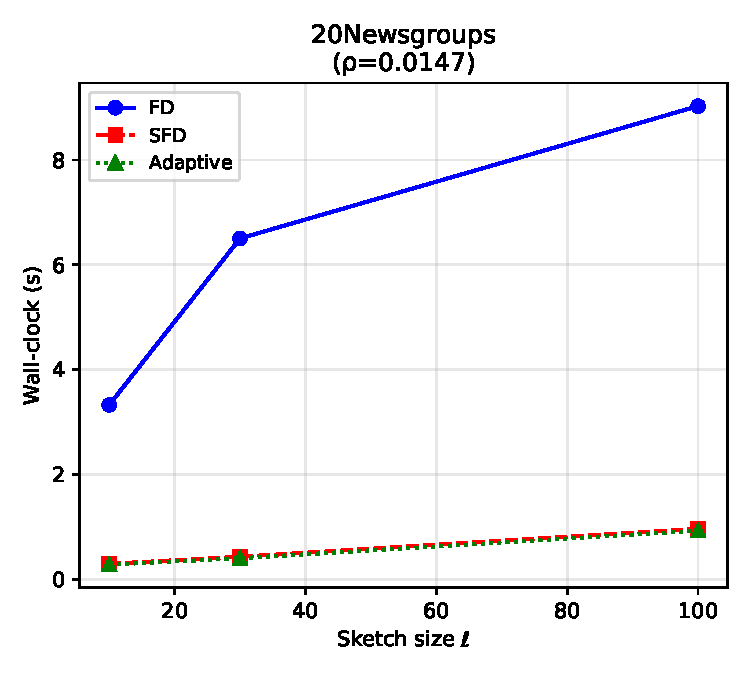
\includegraphics[width=0.95\linewidth]{exp4_real_data.pdf}
  \caption{Wall-clock on MovieLens-1M and 20 Newsgroups at $\ell \in \{10, 30, 100\}$.
    SFD dominates FD by $4\text{--}20\times$; Adaptive matches SFD on five of
    six cells.}
  \label{fig:exp4}
\end{figure}

\subsection{Hardware sensitivity: CPU vs.\ GPU}
\label{ssec:cpu-gpu}

Figure~\ref{fig:exp5} re-runs the density sweep on a Colab T4 GPU using a
CuPy backend. Two effects merit attention. First, GPU FD is roughly
$2\times$ slower than CPU FD at the lowest densities: the FD branch performs
many small $(40 \times 500)$ SVDs, and kernel-launch overhead dominates the
flops. Second, GPU SFD is faster than CPU SFD at every $\rho$ tested, since
its core operations (sparse mat-vecs on a fixed buffer) parallelize cleanly.
The crossover therefore shifts further toward SFD on GPU; a static FD/SFD
threshold would have to be retuned per platform. Adaptive's calibration step
absorbs this shift automatically: the fitted $(\alpha_{\mathrm{fd}}, \beta_{\mathrm{sfd}})$
on T4 differ from M4 by an order of magnitude, biasing the per-batch decision
toward SFD without any user intervention.

\begin{figure}[t]
  \centering
  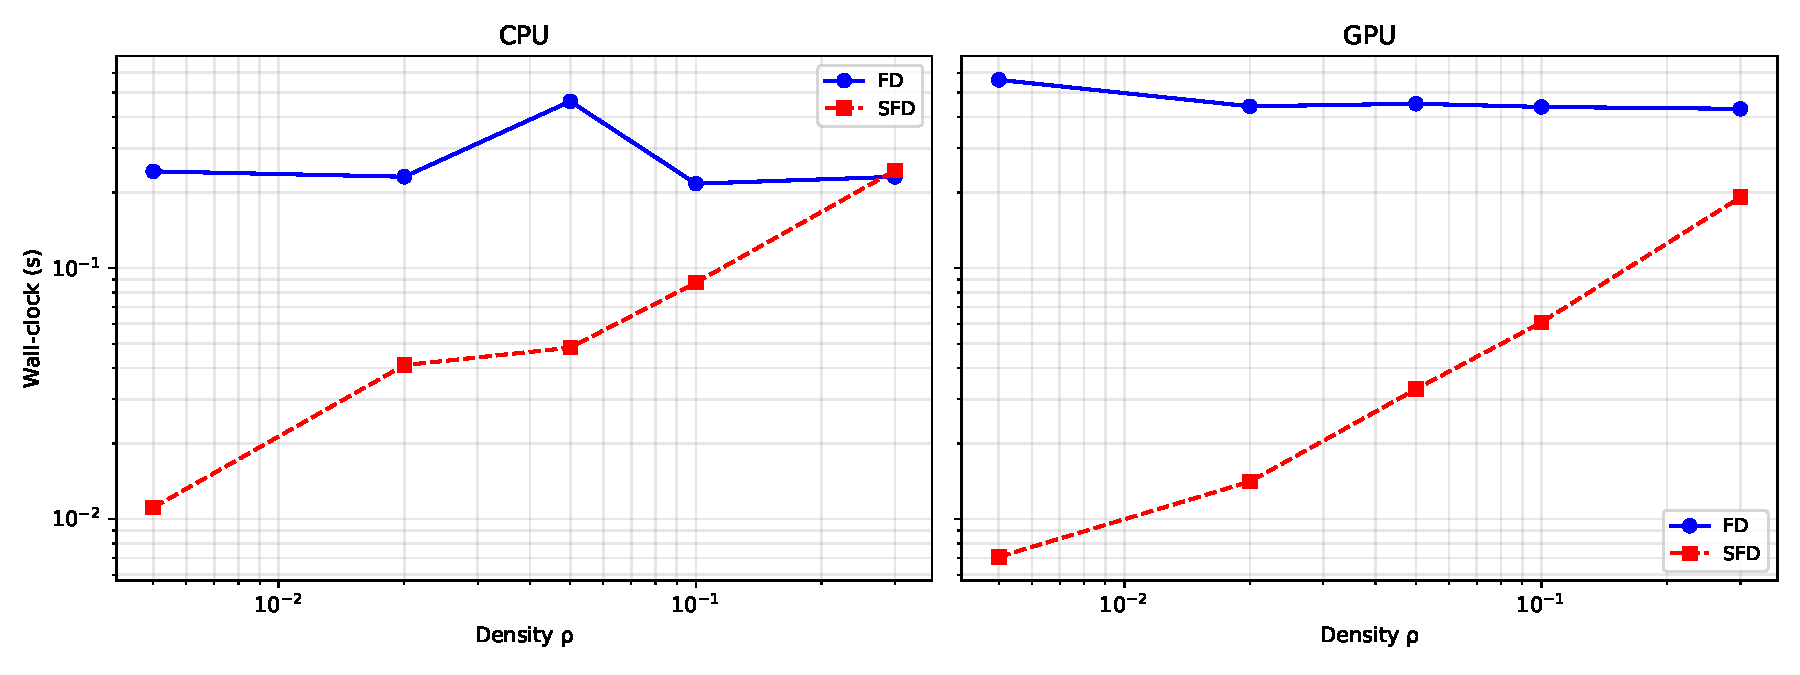
\includegraphics[width=0.7\linewidth]{exp5_cpu_vs_gpu.pdf}
  \caption{Density sweep on CPU (M4) and GPU (Colab T4). GPU FD is slower
    than CPU FD at low $\rho$ due to kernel-launch overhead; GPU SFD is
    faster than CPU SFD at every $\rho$. Adaptive's hardware calibration
    automatically tracks the platform-specific crossover.}
  \label{fig:exp5}
\end{figure}

% ============================================================================
\section{Discussion}
\label{sec:disc}

\textbf{Limitations.} Our cost model is linear in
$(\mathrm{rows}, \mathrm{nnz})$ and ignores cache and memory-bandwidth
effects. This introduces a 5--15\% miss on small sketches and explains the
narrow Adaptive--SFD gap at $\rho \approx 0.3$ in Figure~\ref{fig:exp1}.
Calibration adds a one-time $\sim$30 second cost that amortizes only for
streams larger than $\sim$$10^5$ rows; on shorter streams a static threshold
can match Adaptive in raw wall-clock. The covariance bound degrades
multiplicatively with the fraction of SFD-handled batches, inheriting SFD's
Las Vegas guarantee at worst (Section~\ref{ssec:adaptive-correct}).

\textbf{Outlook.} Two natural extensions arise. First, a third branch using
a sparse random projection could capture the ultra-sparse extreme where
neither exact SVD nor simultaneous iteration is the right tool; the cost
model framework handles new branches uniformly. Second, the calibration
coefficients could be learned online by tracking observed wall-clock per
shrink and updating via exponential averaging, removing the cold-start cost
entirely.

% ============================================================================
\bibliographystyle{plainnat}
\bibliography{refs}

\end{document}
